\clearpage
\section{Parte IV · Desarrollo físico, evidencia humana y cálculos ampliados}
\label{parte-ampliada}

Los capítulos anteriores describen exactamente lo que ejecuta el atlas interactivo.
Esta parte amplía el contexto científico de la monografía de referencia aportada por
los autores. Sus cálculos adicionales se identifican como \emph{análisis en papel}:
el navegador no evalúa un espectro beta, no transporta electrones y no estima una
dosis individual. Esta distinción permite estudiar con profundidad la física de
$^{125}$I y $^{131}$I sin atribuir a la aplicación capacidades que no tiene.

\subsection{Capítulo 7. El sistema biológico y el control experimental}
\label{ampliacion-sistema}

\subsubsection{Incorporación de un análogo de timidina}
El yodo de la iododesoxiuridina, llamada IUdR o IdUrd según la nomenclatura de
cada artículo, forma parte de una molécula análoga a un nucleósido. Durante la
síntesis de ADN, una célula que capta y fosforila el análogo puede incorporarlo
a la cadena naciente. Por tanto, \emph{exposición a actividad en un tubo de cultivo}
y \emph{decaimiento desde la molécula de ADN} no son la misma condición física.
La primera depende de la cantidad en el medio; la segunda exige captación,
metabolismo e incorporación. Tampoco toda célula de una población está en la
misma fase del ciclo ni contiene el mismo número de moléculas marcadas. El
promedio de actividad de la placa puede esconder una distribución desigual entre
células y entre compartimentos de una misma célula.

Whaley y Little emplearon dos líneas linfoblastoides humanas. TK6 era competente
para incorporar el análogo por la vía dependiente de timidina cinasa; SE30 era
deficiente en esa capacidad [1]. Esta diferencia opera como control de
localización, aunque no autoriza a asumir que las líneas son idénticas en todos
los aspectos. Los autores consideraron explicaciones alternativas, como
sensibilidades radiológicas o sensibilización por el análogo, y concluyeron que
no explicaban la diferencia observada [1]. En particular, el $^{125}$I--IdUrd
incorporado fue muy tóxico y mutagénico en TK6, mientras una actividad semejante
en el medio externo casi no produjo efecto en las células deficientes. Para
$^{131}$I--IdUrd se comunicó en TK6 una pendiente de mutantes inducidos en
\emph{hprt} de $0,45\times10^{-6}$ por cGy de dosis nuclear; se encontraron
pocas mutaciones en SE30 hasta 38 cGy provenientes de decaimientos del medio
[1]. No se publicó allí una tasa universal de mutación de todo el genoma.

El resultado permite una inferencia física importante. Si dos preparaciones
tienen actividad macroscópica comparable, pero una inicia emisiones directamente
en el ADN, la topología microscópica de la fuente modifica la probabilidad de
que una traza intercepte moléculas relevantes. No se deduce que cada desintegración
cause una lesión, que cada lesión se convierta en mutación ni que los valores
obtenidos en cultivo puedan aplicarse sin más a pacientes.

\subsubsection{Qué mide HPRT y qué significa un clon resistente}
La hipoxantina--guanina fosforribosiltransferasa participa en la vía de rescate de
purinas. La selección con 6-tioguanina puede enriquecer células que perdieron
función HPRT y sobreviven bajo las condiciones del ensayo. La timidina cinasa
interviene en la incorporación del análogo: no debe confundirse con HPRT,
que es el \emph{locus de lectura} de mutación. Una colonia resistente es un
resultado funcional de proliferación y selección, no una fotografía directa de
una rotura doble en el instante del decaimiento. Se requiere tiempo de expresión
fenotípica; además hay que corregir eficiencia de clonación, supervivencia,
mutantes de fondo y condiciones de cultivo. Una muestra con muy pocas células
vivas puede producir pocas colonias aun si el daño inicial fue intenso.

Sea $n$ el número de células clonables sembradas por pocillo y $f$ la
probabilidad efectiva de que una de ellas dé un clon resistente. Si los
eventos son independientes y raros, el número de clones por pocillo se aproxima
por una variable de Poisson de media $nf$. Entonces
\begin{align}
P(K=k)&=\frac{(nf)^k}{k!}e^{-nf},\\
P(K=0)&=e^{-nf},\\
f&=-\frac{\ln P(K=0)}{n}.
\end{align}
Esta identidad muestra por qué contar sólo pocillos positivos no equivale a
contar mutantes: un pocillo puede contener más de un clon. Si la fracción vacía
es $P_0=0,90$ y se siembran $10^4$ células clonables por pocillo, el cálculo
ilustrativo da $f=-\ln(0,90)/10^4\simeq1,054\times10^{-5}$.
No se afirma que esos números pertenezcan a Whaley y Little; únicamente se
explica el principio estadístico del ensayo. Con datos reales conviene usar
el procedimiento de clonación y los controles publicados por sus autores.

\subsubsection{Una escalera de inferencia biológica}
Hay por lo menos cuatro niveles distintos: la localización del radionúclido,
una ionización o lesión inicial, una respuesta celular y una mutación fijada
en descendientes. A nivel citogenético, una aberración cromosómica es un
quinto resultado que no se identifica automáticamente con una mutación HPRT.
Las imágenes de la web ilustran esta secuencia, pero no la observan ni la
calculan desde primeros principios. En las dos escenas elegidas para la
exposición, la regla de diez pares de bases define sólo un \emph{criterio de
clasificación} para el Monte Carlo, y la pendiente HPRT es un resultado
experimental de una condición precisa [1]. La primera permite razonar sobre
daño agrupado; la segunda obliga a preguntar qué sobreviven y qué se cuenta.

\clearpage
\subsection{Capítulo 8. Captura electrónica, conversión interna y relojes nucleares}
\label{ampliacion-captura}

\subsubsection{Transformación y cantidades conservadas}
En captura electrónica, un protón nuclear y un electrón atómico se convierten
en neutrón y neutrino electrónico por interacción débil cargada. El esquema
de nucleones y el nuclear se escriben
\begin{align}
p+e^-&\longrightarrow n+\nu_e,\\
{}^{125}_{53}\mathrm I+e^-_{\rm ligado}
 &\longrightarrow{}^{125}_{52}\mathrm{Te}^{*}+\nu_e.
\end{align}
El número másico continúa siendo 125; la carga del núcleo pasa de $+53e$ a
$+52e$. Si se incluye el electrón inicial, la carga total del sistema es la
misma a ambos lados. El número leptónico electrónico inicial $+1$ aparece en
el neutrino final. En el vértice quark subyacente un quark $u$ pasa a $d$;
esa descripción explica la reducción de la carga de un nucleón, pero no
autoriza a imaginar una colisión mecánica simple dentro de la célula.

Definimos el valor energético con masas de \emph{átomos neutros en sus estados
fundamentales}, y representamos explícitamente una rama con excitación nuclear
$E_*$ y captura desde una capa de energía de enlace $B_i$:
\begin{align}
Q_{\rm EC}&=\big[M_a({}^{125}\mathrm I)-M_a({}^{125}\mathrm{Te})\big]c^2,\\
Q_{\rm EC}&\simeq E_{\nu,i}+E_*+B_i+T_R+\delta_i,\\
E_{\nu,i}&\simeq Q_{\rm EC}-E_*-B_i-T_R-\delta_i.
\end{align}
El término $\delta_i$ recuerda las correcciones atómicas y la convención
precisa con la que se contabilizan vacantes y masas. No se reparte $Q_{\rm EC}$
por igual entre los electrones Auger. La captura deja una vacante en la nube
electrónica; una transición desde otra capa puede emitir un rayo X
característico o transferir la energía a un electrón expulsado. También la
desexcitación del $^{125}$Te puede expulsar un electrón orbital por
\emph{conversión interna}, creando vacantes adicionales. Según la ficha IAEA,
la semivida del $^{125}$I es 59,408 d y la transición gamma de unos 35,49 keV
tiene intensidad 6,68\%; el resto de la desexcitación de ese estado está
fuertemente convertido [6]. La energía de la línea gamma no es la energía
común de los electrones Auger.

\subsubsection{Retroceso: una escala pequeña y su significado}
En una estimación que omite los momentos de otras emisiones, el neutrino lleva
$p_\nu c\simeq E_\nu$ y el núcleo hijo recibe momento opuesto. Para una masa
de reposo $M_R c^2$ mucho mayor que la energía liberada,
\begin{align}
T_R&=\frac{p_R^2}{2M_R}\simeq\frac{E_\nu^2}{2M_Rc^2},\\
M_Rc^2&\simeq125(931{,}494\;\mathrm{MeV})
       =1{,}16437\times10^8\;\mathrm{keV}.
\end{align}
Si se \emph{elige sólo a modo de ejemplo} $E_\nu=150$ keV, se obtiene
\[
T_R\simeq\frac{(150\,\mathrm{keV})^2}
 {2(1{,}16437\times10^8\,\mathrm{keV})}
 =9{,}66\times10^{-5}\,\mathrm{keV}\simeq0{,}0966\,\mathrm{eV}.
\]
El cálculo de orden de magnitud descarta atribuir la eficacia local
principalmente a un gran retroceso del núcleo. Para describir el daño químico
se necesitarían la cascada electrónica, el ambiente acuoso y el transporte
de electrones secundarios; la web reemplaza todo ello por un perfil de
probabilidad declarado.

\subsubsection{Derivación de semivida, actividad y una ventana celular}
Para un conjunto de núcleos independientes con tasa de decaimiento constante
$\lambda$, la esperanza de pérdidas en $dt$ es $\lambda N(t)dt$ y
\begin{align}
\frac{dN}{dt}&=-\lambda N,&
N(t)&=N_0 e^{-\lambda t},&
A(t)&=\lambda N(t),\\
\lambda&=\frac{\ln2}{T_{1/2}},&
F_{\rm dec}(t)&=1-e^{-\lambda t}.
\end{align}
La tasa $\lambda$ tiene unidades de tiempo inverso. Cuando $t$ está
en segundos, $A$ se mide en Bq. Antes de dividir Bq por una tasa en
d$^{-1}$, ésta se convierte a s$^{-1}$. La figura muestra el reloj
nuclear; la permanencia en ADN añade otro reloj.

\begin{figure}[htbp]\centering
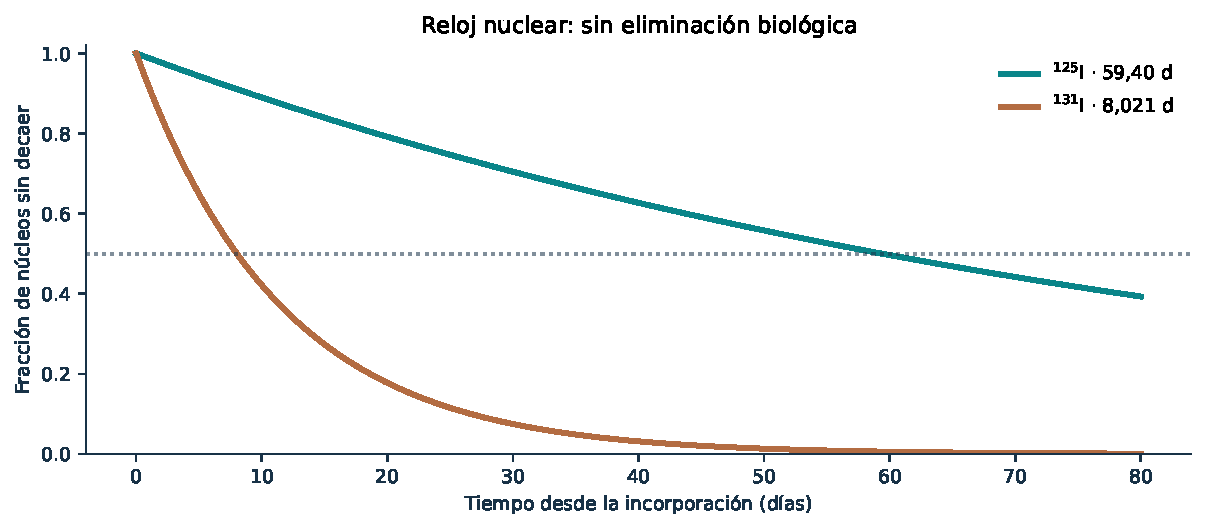
\includegraphics[width=.92\linewidth]{figuras_monografia/06_semividas_fisicas.pdf}
\caption{Supervivencia física de $^{125}$I y $^{131}$I calculada con las semividas
indicadas. No incorpora captación ni salida biológica.}\end{figure}

Con $T_{1/2}(^{125}\mathrm I)=59,40$ d y $t=18$ h $=0,75$ d,
$\lambda_{125}=0,011669$ d$^{-1}$ y
$F_{125}(0,75)=1-2^{-0,75/59,40}\simeq0,008714$.
Con $T_{1/2}(^{131}\mathrm I)=8,021$ d [7],
$\lambda_{131}=0,086416$ d$^{-1}$ y
$F_{131}(0,75)\simeq0,06275$. En idéntica ventana y para igual número
inicial de átomos, la fracción física que decae es mayor para $^{131}$I.
Ello no establece la dosis de una célula: los dos tipos de radiación y sus
geometrías de deposición difieren, y la cantidad incorporada podría ser distinta.

\clearpage
\subsection{Capítulo 9. Espectro beta de $^{131}$I y alcance de la aproximación}
\label{ampliacion-beta}

\subsubsection{Tres cuerpos y espectro continuo}
En el decaimiento beta menos, un neutrón se transforma en protón y se producen
un electrón y un antineutrino electrónico:
\begin{align}
n&\longrightarrow p+e^-+\bar\nu_e,\\
{}^{131}_{53}\mathrm I&\longrightarrow
 {}^{131}_{54}\mathrm{Xe}^{*}+e^-+\bar\nu_e.
\end{align}
La suma de energía cinética del electrón, del antineutrino y del retroceso,
más la excitación nuclear, iguala el valor $Q_\beta$. A diferencia de una
transición de dos cuerpos con masa hija fijada, el electrón y el antineutrino
comparten energía en una familia continua de configuraciones permitidas por
conservación de energía y momento. Si el núcleo hijo queda en distintos niveles,
cambia la energía final disponible para esa rama. Por ello \emph{un espectro de
una sola rama} no equivale al espectro total del $^{131}$I.

Para una rama permitida con endpoint $T_0$ y neutrino de masa despreciable,
una forma pedagógica de la densidad sin correcciones radiativas es
\begin{align}
\widetilde s(T)&=F(Z,T)\,p(T)\,[T+m_ec^2]\,(T_0-T)^2,\\
p(T)c&=\sqrt{T\big(T+2m_ec^2\big)},\qquad 0\leq T\leq T_0,\\
s(T)&=\frac{\widetilde s(T)}{\int_0^{T_0}\widetilde s(u)\,du},\qquad
C(T)=\int_0^T s(u)\,du.
\end{align}
El factor $(T_0-T)^2$ procede del espacio de fases aproximado del
antineutrino; $p(T)[T+m_ec^2]$ es la parte cinemática electrónica. La
función de Fermi $F(Z,T)$ corrige la interacción de Coulomb con el núcleo
hijo. En la figura se fija deliberadamente $F=1$ para mostrar solamente la
forma cinemática. El endpoint de 606,3 keV corresponde a una rama intensa
del $^{131}$I; no se debe confundir con la máxima energía de todas las ramas
ni con la energía media de sus electrones [15].

\begin{figure}[htbp]\centering
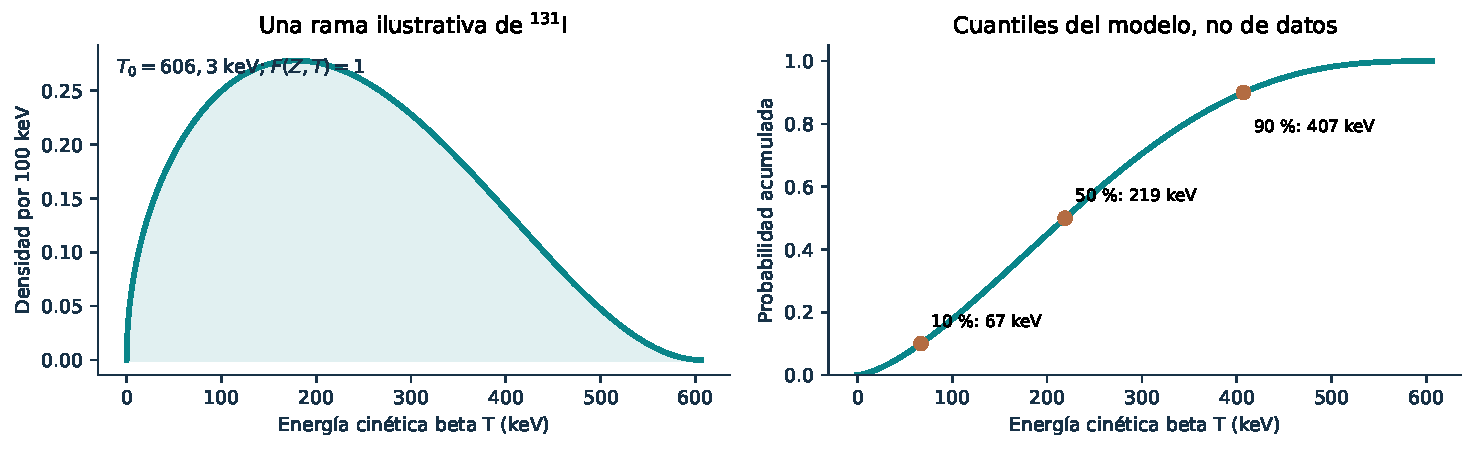
\includegraphics[width=.97\linewidth]{figuras_monografia/05_beta_modelo.pdf}
\caption{Espectro beta de una rama permitida y su distribución acumulada,
normalizados numéricamente con $T_0=606,3$ keV y $F=1$. Curvas derivadas,
no espectros medidos ni resultados de la simulación web.}\end{figure}

El área bajo $s(T)$ se fuerza a uno por integración trapezoidal. La CDF
comienza en cero y termina en uno por construcción. El cálculo arroja
cuantiles aproximados $T_{10}\simeq67$ keV,
$T_{50}\simeq219$ keV y $T_{90}\simeq407$ keV para \emph{este modelo}.
Cambiar la función de Fermi, la forma de transición, las ramas y sus
intensidades cambia esos valores. Su utilidad es conceptual: ni siquiera
una rama con endpoint fijo emite siempre electrones con la misma energía.
La gráfica no debe insertarse en una estimación de dosis de paciente como si
fuera una evaluación nuclear completa.

\subsubsection{Conservación y cinemática de un electrón de prueba}
La relación relativista entre energía total y momento es
\[
E^2=(pc)^2+(m_ec^2)^2,\qquad E=T+m_ec^2,\qquad
pc=\sqrt{T(T+2m_ec^2)}.
\]
Para $T=200$ keV y $m_ec^2=510,999$ keV,
\[
pc=\sqrt{200(200+2\cdot510,999)}\,\mathrm{keV}
\simeq494,37\,\mathrm{keV},
\qquad p\simeq494,37\,\mathrm{keV}/c.
\]
Ese número es el momento de \emph{un electrón supuesto} de 200 keV; no es
un momento representativo de todas las ramas. La presencia del antineutrino
es necesaria para el balance energético y leptónico. La emisión gamma desde
estados excitados de $^{131}$Xe pertenece a la desexcitación posterior y
tampoco se identifica con la energía del electrón beta.

\subsubsection{Relación con la escena interactiva}
La escena 01 de la web muestra captura y relajación para $^{125}$I; la escena
02 contrasta los dos relojes físicos y una salida hipotética. No hay una
escena que muestree el espectro beta de la figura: éste se incluye para
cubrir la física subatómica de $^{131}$I exigida por la monografía previa.
La escena 06 emplea una pendiente experimental de mutantes, sin obtenerla
por integración del espectro. No existe en el código una cadena de transporte
de partículas que conecte cada $T$ con un depósito energético local.

\clearpage
\subsection{Capítulo 10. Microdosimetría: volumen, distancia y definición de dosis}
\label{ampliacion-micro}

\subsubsection{De la energía a un promedio geométrico}
La dosis absorbida macroscópica es $D=d\bar\varepsilon/dm$, medida en
Gy $=\mathrm{J}/\mathrm{kg}$. Con un depósito supuesto $E_{\rm dep}$ uniforme
en una esfera acuosa de radio $r$ y densidad $\rho$, un promedio formal es
\begin{align}
V(r)&=\frac43\pi r^3,\\
m(r)&=\rho V(r),\\
D_{\rm esfera}(r)&=\frac{E_{\rm dep}}{\rho(4\pi r^3/3)}.
\end{align}
Si la energía y la densidad permanecen constantes, duplicar $r$ multiplica
el denominador por ocho y divide el promedio por ocho. Esto ilustra por qué
una energía pequeña puede corresponder a un cociente enorme si la masa
elegida es nanométrica. No significa que una desintegración deposite toda
su energía dentro de una esfera homogénea ni que ese cociente sea la dosis
celular medida.

Para reproducir el ejemplo del cuaderno de referencia, \emph{se supone}
$E_{\rm dep}=16,51$ keV y $r=10$ nm en agua de densidad
$\rho=1000\;\mathrm{kg,m^{-3}}$. Se convierten todas las unidades antes
de dividir:
\begin{align}
E_{\rm dep}&=16,51\times10^3\;\mathrm{eV}
  \times1,602176634\times10^{-19}\;\mathrm{J/eV}
  =2,64519\times10^{-15}\;\mathrm J,\\
r&=10\;\mathrm{nm}=10^{-8}\;\mathrm m,\\
V&=\frac43\pi(10^{-8}\;\mathrm m)^3
  =4,18879\times10^{-24}\;\mathrm{m^3},\\
m&=(1000\;\mathrm{kg/m^3})V
  =4,18879\times10^{-21}\;\mathrm{kg},\\
D_{\rm esfera}&=\frac{2,64519\times10^{-15}\;\mathrm J}
 {4,18879\times10^{-21}\;\mathrm{kg}}
  =6,315\times10^5\;\mathrm{Gy}.
\end{align}
La magnitud extrema procede \emph{del volumen escogido}, no de una dosis
medida en el núcleo o en el cuerpo. Si sólo la fracción $g$ de la energía
queda allí, el promedio sería $gD_{\rm esfera}$, con $0\leq g\leq1$;
en una traza real la distribución es heterogénea y no equivale a una esfera
uniforme. La figura permite inspeccionar el exponente $r^{-3}$.

\begin{figure}[htbp]\centering
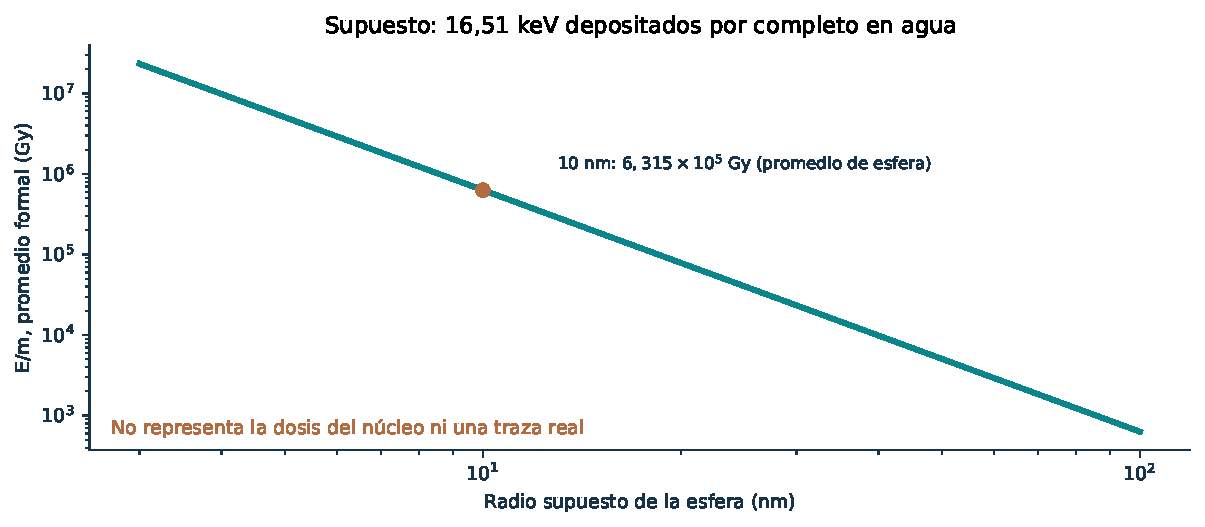
\includegraphics[width=.93\linewidth]{figuras_monografia/07_esfera_energia.pdf}
\caption{Cociente $E/m$ para una esfera de agua con energía supuestamente
depositada de 16,51 keV. El radio es una elección del ejemplo; el eje vertical
no representa dosimetría clínica ni una traza electrónica calculada.}\end{figure}

\subsubsection{Qué representa y qué no representa la distancia del modelo}
En la web, cada sitio $j$ de las dos hebras de una hélice B ideal de 60 pares
de bases tiene una posición $\mathbf x_j$. La fuente se coloca en
$\mathbf s$; se calcula $r_j=\|\mathbf x_j-\mathbf s\|$. Para parámetros
supuestos $\mu$ y $\ell$, la probabilidad de una oportunidad de lesión es
\[
p_j=1-\exp\!\left[-\mu\exp(-r_j/\ell)\right].
\]
Se puede derivar suponiendo que el número $K_j$ de oportunidades locales
es Poisson de media $\mu\exp(-r_j/\ell)$; entonces
$P(K_j\geq1)=1-P(K_j=0)=p_j$. El parámetro $\mu$ es adimensional y $\ell$
se mide en nm. El factor $\exp(-r_j/\ell)$ es una elección fenomenológica,
no una ley del frenado de electrones de Auger. El código toma sorteos
Bernoulli independientes por sitio; las correlaciones químicas verdaderas
quedan fuera de esta aproximación. El modelo de esfera de esta sección y el
modelo de Bernoulli del navegador son \emph{dos ilustraciones diferentes}:
no hay conversión en el programa de Gy por esfera a $\mu$ o $\ell$.

Una SSB operacional se marca cuando el sorteo en un sitio de una hebra
produce lesión. Una DSB operacional requiere dos marcas en hebras opuestas
cuya separación longitudinal en índices sea como máximo diez pares de bases.
Diez pares corresponden a unos $3,4$ nm a lo largo del eje de la hélice
ideal si se usa $0,34$ nm por par, pero la distancia tridimensional entre
sitios no es necesariamente $3,4$ nm. El número diez es una convención
del ejercicio, no un umbral biológico universal. El gráfico de sensibilidad
de la parte anterior muestra que variar $\mu$ y $\ell$ altera mucho las
frecuencias, razón por la cual no se interpretan como predicciones
experimentales de DSB por decaimiento [2].

\subsubsection{De microgeometría a una medición válida}
Una simulación de transporte defendible necesitaría el espectro de electrones
Auger y de conversión interna de cada rama, velocidades y direcciones,
colisiones inelásticas y elásticas, electrones secundarios, estado de
ionización de la molécula, agua y oxígeno, radicales, estructura molecular
del ADN y tiempos químicos. Después habría que definir lesiones,
compararlas con experimentos y propagar incertidumbres. Las gráficas de
este documento cumplen otra función: muestran cómo una \emph{hipótesis
espacial explícita} afecta un resultado, y permiten que otra persona
recalcule exactamente las mismas curvas con los archivos de código.

\clearpage
\subsection{Capítulo 11. De la actividad incorporada al número esperado de decaimientos}
\label{ampliacion-compartimentos}

\subsubsection{Contabilidad de actividad y fracciones}
Sean $A_0$ Bq administrados en un contexto hipotético, y $f_T,f_C,f_N,f_D$
las fracciones condicionales sucesivas que alcanzan tumor, célula, núcleo
y ADN. Un producto $f=f_Tf_Cf_Nf_D$ es una \emph{representación de
contabilidad} sólo si cada factor fue definido con el denominador correcto.
No se ha medido ninguno de ellos en el sitio web. El número de núcleos
iniciales asociados a ADN se escribiría
\[
N_{D,0}=f\frac{A_0}{\lambda},
\qquad [A_0]=\mathrm{s^{-1}},\quad[\lambda]=\mathrm{s^{-1}}.
\]
No hay que confundir $f$ con la probabilidad de mutación $f_{\rm HPRT}$.
Si la actividad se mide después de la incorporación, se usa la actividad
de ese compartimento y no se multiplica otra vez por las fracciones de
captación. Esta aclaración evita contar la incorporación dos veces.

\subsubsection{Dos riesgos competitivos y su derivación}
Sea $\lambda$ la tasa nuclear y $k$ una tasa de salida del compartimento
ADN, ambas constantes en el ejemplo. La probabilidad de que un núcleo
continúe allí y sin decaer hasta $t$ satisface
\begin{align}
S_D(t)&=\exp[-(\lambda+k)t],\\
P_{\rm dec\,en\,ADN}(t)
 &=\int_0^t\lambda S_D(u)\,du
 =\frac{\lambda}{\lambda+k}
    \bigl(1-e^{-(\lambda+k)t}\bigr),\\
P_{\rm sale}(t)
 &=\frac{k}{\lambda+k}
    \bigl(1-e^{-(\lambda+k)t}\bigr).
\end{align}
La suma $P_{\rm dec\,en\,ADN}(t)+P_{\rm sale}(t)+S_D(t)=1$ es una
prueba de conservación. A tiempos largos, la fracción que decae antes de
salir es $\lambda/(\lambda+k)$. Si $k=0$, tiende a uno; si
$k\gg\lambda$, tiende a cero. La \emph{semivida efectiva} de la población
que permanece en el compartimento es $T_{1/2,\rm ef}=\ln2/(\lambda+k)$.
Esto no reemplaza la semivida nuclear: una molécula que sale sigue
conteniendo un radionúclido con la misma tasa de desintegración, pero ya
no decae en la ubicación modelada.

\begin{figure}[htbp]\centering
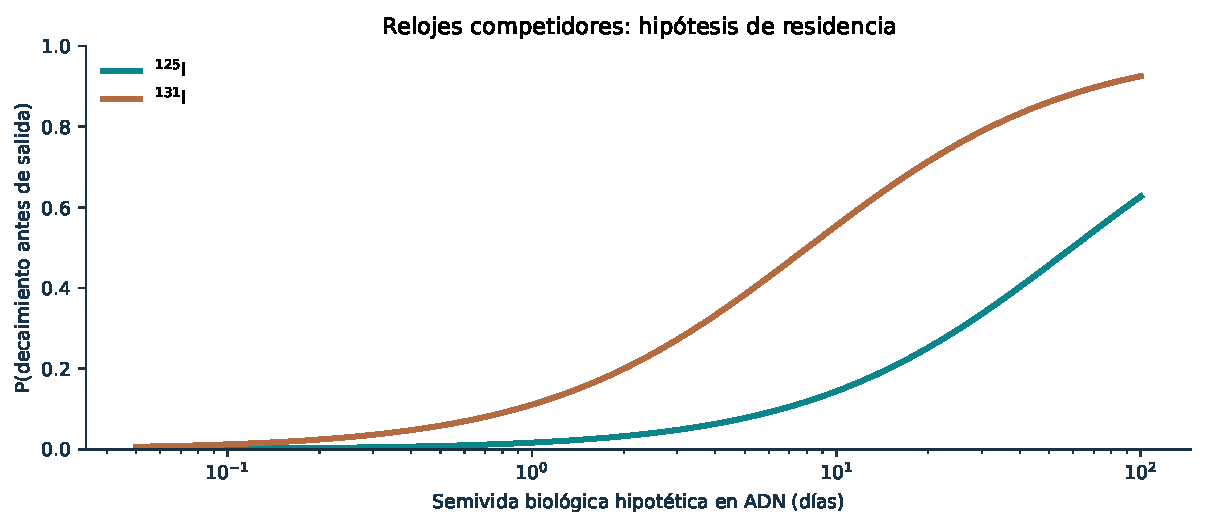
\includegraphics[width=.92\linewidth]{figuras_monografia/08_competencia_biologica.pdf}
\caption{Probabilidad límite de decaer antes de abandonar ADN frente a una
semivida biológica elegida. La curva es una consecuencia del modelo de riesgos
competitivos; no mide retención en TK6 ni biocinética humana.}\end{figure}

La escena 02 implementa precisamente esta competencia. Si el usuario mueve
el deslizador de salida, modifica $k$ y ve un resultado condicional del
modelo. La figura no permite seleccionar una dosis prescrita ni conocer
retención real. En un paciente $k$ podría variar con el tiempo, la célula,
la división y el metabolismo; haría falta un modelo biocinético validado
para remplazar la constante hipotética.

\subsubsection{Propagación de una incertidumbre elemental}
Para $P_\infty=\lambda/(\lambda+k)$,
\[
\frac{\partial P_\infty}{\partial k}
 =-\frac{\lambda}{(\lambda+k)^2},\qquad
\frac{\partial P_\infty}{\partial\lambda}
 =\frac{k}{(\lambda+k)^2}.
\]
Si $k$ se incrementa, la probabilidad disminuye; si $\lambda$ aumenta
manteniendo $k$, aumenta. Bajo errores pequeños e independientes, una
propagación lineal sería
\[
\sigma_P^2\simeq
 \left(\frac{\partial P}{\partial\lambda}\sigma_\lambda\right)^2+
 \left(\frac{\partial P}{\partial k}\sigma_k\right)^2.
\]
El texto no da un valor numérico de $\sigma_k$, porque no hay medición de
retención en el proyecto. Fijar arbitrariamente uno haría parecer calibrado
un ejemplo que no lo está. El error estándar binomial reportado por la
escena de DSB, por su parte, cuantifica sólo variación del muestreo con
parámetros fijos, no esta incertidumbre de modelo.

\clearpage
\subsection{Capítulo 12. Resultados externos en material humano}
\label{ampliacion-evidencia}

\subsubsection{Linfocitos y la importancia de leer el corrigendum}
El estudio de Schmitz y colaboradores expuso linfocitos humanos de sangre
periférica al $^{125}$I--UdR y examinó aberraciones cromatídicas y muerte
celular [12]. Su población marcada era heterogénea: el resumen público
describe cerca de 40\% de células muy marcadas, 20\% moderadamente
marcadas y 40\% sin marcar. Un promedio de actividad puede por tanto
ocultar exposiciones muy diferentes dentro del mismo cultivo. La
publicación de 2016 corrigió expresamente una inferencia numérica de la
versión de 2015: con nueve experimentos, sus datos indicaron \emph{en
promedio unas 250 desintegraciones por aberración cromosómica} en las
condiciones medidas [9]. Así, un ejemplo aritmético de 2500
desintegraciones produciría una esperanza de 10 aberraciones bajo una
extrapolación lineal del cociente, \emph{no} diez DSB observadas y tampoco
diez mutaciones HPRT. La heterogeneidad celular y la selección de
metafases limitan la traslación directa. Se cita la corrección junto al
artículo original para no repetir la interpretación retractada.

\subsubsection{Biodistribución y localización en pacientes}
Mariani y colaboradores estudiaron diez personas con cáncer colorrectal
después de una inyección intratumoral de $^{125}$I--UdR de 0,24 a
3,9 MBq antes de cirugía [13]. Midieron actividad en tumor y tejidos
vecinos y usaron microautoradiografía de cortes resecados. El resumen
publicado informa que esta última mostró localización en núcleos de
células tumorales humanas. Esto responde una pregunta distinta a la del
ensayo HPRT: confirma que la molécula puede alcanzar la ubicación
celular relevante bajo esa vía concreta, pero no mide con ello una tasa
de mutación en un paciente. Además, la distribución intratumoral y la
incorporación normal no son homogéneas por definición. La cifra media
de actividad por gramo y la relación tumor/tejido vecino del artículo
no deben tratarse como fracciones universales del modelo de la web.

\subsubsection{Primer caso terapéutico y límites de inferencia}
Rebischung y colaboradores publicaron en 2008 una primera experiencia
humana de administración intratecal de $^{125}$I--UdR junto con
metotrexato para meningitis neoplásica resistente [14]. Un caso permite
discutir factibilidad, seguimiento y preguntas de seguridad; no permite
aislar el efecto del radiofármaco respecto al metotrexato ni estimar
eficacia general. En esta monografía sirve de puente entre un mecanismo
en cultivo y el tipo de problemas que aparecen en seres humanos. No se
infieren de él indicaciones, dosis clínicas, probabilidad personal de
mutación o beneficio terapéutico. El foco experimental cuantitativo
continúa siendo Whaley y Little [1].

\begin{table}[htbp]\centering\small
\begin{tabularx}{\linewidth}{@{}p{.19\linewidth}p{.31\linewidth}X@{}}
\toprule Fuente & Observación pertinente & Inferencia autorizada \\\midrule
Whaley y Little [1] & Mutantes HPRT y supervivencia, TK6/SE30 & Eficacia relativa de decaimientos incorporados en células humanas bajo el ensayo. \\
Schmitz et al. [12,9] & Aberraciones en linfocitos y corrección de 250 desintegraciones por aberración & Un endpoint citogenético y su cifra corregida, no DSB por desintegración. \\
Mariani et al. [13] & Microautoradiografía tras inyección en diez pacientes & Localización nuclear tumoral bajo una ruta específica, no tasa clínica de mutaciones. \\
Rebischung et al. [14] & Primer caso intratecal con tratamiento combinado & Factibilidad y preguntas clínicas; no eficacia general ni atribución aislada. \\\bottomrule
\end{tabularx}
\caption{Cuatro niveles de evidencia que no se convierten unos en otros por una sola ecuación.}
\end{table}

La figura de la escena 06 representa de manera pedagógica una pendiente de
mutantes publicada [1]. La escena 04 produce una frecuencia de DSB
\emph{simulada} a partir de probabilidades supuestas. Nunca se ajustó
$\mu$ hasta que la frecuencia de DSB coincidiera con los 250 decaimientos
por aberración de un experimento distinto. Hacerlo sin un modelo de
reparación y observación de cromosomas equivaldría a identificar endpoints
incompatibles.

\clearpage
\subsection{Capítulo 13. Cálculos resueltos y comprobaciones dimensionales}
\label{ampliacion-ejercicios}

\subsubsection{Problema 1: un intervalo de dieciocho horas}
Se pregunta qué fracción de un conjunto de $N_0$ átomos \emph{incorporados y
retenidos por hipótesis} decae en dieciocho horas. Primero se expresa el
tiempo en la misma unidad de la semivida: $18\,\mathrm h=18/24=0,75$ d.
Después se calcula $\lambda=\ln2/T_{1/2}$, con dimensión d$^{-1}$.
Finalmente se evalúa $1-\exp(-\lambda t)$. Usando $59,40$ y $8,021$ d,
respectivamente, se obtiene
\begin{align}
\lambda_{125}&=\frac{0,693147}{59,40\;\mathrm d}
  \simeq0,0116691\;\mathrm d^{-1},\\
F_{125}(18\,\mathrm h)&=1-e^{-0,0116691(0,75)}
  \simeq0,008714\simeq0,8714\%,\\
\lambda_{131}&=\frac{0,693147}{8,021\;\mathrm d}
  \simeq0,086416\;\mathrm d^{-1},\\
F_{131}(18\,\mathrm h)&=1-e^{-0,086416(0,75)}
  \simeq0,06275\simeq6,275\%.
\end{align}
Cada exponente es adimensional. El resultado $F_{131}/F_{125}\simeq7,20$
compara \emph{fracciones de átomos iniciales} que decaen, no dosis,
mutaciones ni actividades administradas. Si se usara una semivida tabulada
de $8,0252$ d como en el cuaderno anterior, habría una diferencia pequeña
en las últimas cifras; aquí se mantiene $8,021$ d de ICRP [7] para coincidir
con el programa. Una semivida biológica distinta modificaría el número de
decaimientos que tienen lugar antes de salir del ADN.

\subsubsection{Problema 2: convertir una actividad en núcleos}
Supóngase una actividad inicial de $A_0=1000$ Bq de $^{125}$I en un
compartimento \emph{hipotético}. Una actividad de 1000 Bq significa
1000 desintegraciones esperadas por segundo en ese instante. Convertimos
la constante nuclear:
\begin{align}
T_{1/2}&=59,40\;\mathrm d\times86400\;\mathrm{s/d}
  =5\,132\,160\;\mathrm s,\\
\lambda&=\frac{0,693147}{5\,132\,160\;\mathrm s}
  \simeq1,3506\times10^{-7}\;\mathrm{s^{-1}},\\
N_0&=\frac{A_0}{\lambda}
  \simeq\frac{1000\;\mathrm{s^{-1}}}{1,3506\times10^{-7}\;\mathrm{s^{-1}}}
  \simeq7,40\times10^9\;\text{núcleos}.
\end{align}
Este número no dice cuántos átomos están en ADN: para ello habría que medir
la actividad de esa fracción o introducir una fracción de incorporación
con incertidumbre. La igualdad $A=\lambda N$ relaciona una esperanza
instantánea con la cantidad de átomos, no una cuenta exacta de eventos
individuales en un intervalo corto.

\subsubsection{Problema 3: pendiente HPRT y cambio de unidades}
La pendiente experimental de $^{131}$I--IdUrd en TK6 se reporta como
$\alpha=0,45\times10^{-6}\,\mathrm{cGy}^{-1}$ de mutantes inducidos por
célula clonable [1]. Como $1\,\mathrm{Gy}=100\,\mathrm{cGy}$, el mismo
producto $\alpha D$ debe mantenerse al cambiar de unidad:
\[
\alpha=45\times10^{-6}\,\mathrm{Gy}^{-1}.
\]
Si se \emph{extiende linealmente} la pendiente hasta $D=38$ cGy
$=0,38$ Gy,
\begin{align}
\Delta f&=(0,45\times10^{-6}\,\mathrm{cGy}^{-1})
                 (38\,\mathrm{cGy})\\
 &=17,1\times10^{-6}
 =17,1\;\text{mutantes inducidos por millón de células clonables}.
\end{align}
El mismo resultado surge de $(45\times10^{-6}\,\mathrm{Gy}^{-1})(0,38\,
\mathrm{Gy})$. Los 38 cGy en el resumen del artículo describen el límite
de dosis mencionado para \emph{SE30} con decaimientos en el medio; no
constituyen una medida directa de TK6 a ese punto. Así, $17,1$ es una
extrapolación aritmética expresamente rotulada, no una observación [1].

\subsubsection{Problema 4: del valor esperado al conteo de pocillos}
Si $n$ células clonables por pocillo tienen frecuencia efectiva
$f(D)=f_0+\alpha D$ y se aceptan los supuestos de rareza e independencia,
$Y\sim\mathrm{Poisson}(nf(D))$. Para $m$ pocillos independientes,
la suma $Y_\mathrm{total}$ sería Poisson de media $mnf(D)$.
Si una población sólo tiene $n=1000$ células clonables por pocillo,
$f_0=10\times10^{-6}$ es un fondo \emph{elegido} y se usa
$D=38$ cGy como ejemplo aritmético, entonces
\[
f(D)=27,1\times10^{-6},\quad
E[Y]=0,0271,\quad P(Y=0)=e^{-0,0271}\simeq0,9733.
\]
Es posible que la mayoría de pocillos no tenga mutantes resistentes
incluso con una frecuencia inducida distinta de cero. Variar el número
de pocillos cambia la precisión estadística, no la frecuencia biológica.
En la aplicación el fondo, el número de células y el generador aleatorio
son controles del escenario, no valores medidos por Whaley y Little.

\subsubsection{Problema 5: un intervalo de incertidumbre del Monte Carlo}
Si $n_\mathrm{sim}$ desintegraciones simuladas generan $k$ sucesos DSB,
$\widehat p=k/n_\mathrm{sim}$ y el error estándar binomial aproximado es
\[
\operatorname{SE}(\widehat p)=
\sqrt{\frac{\widehat p(1-\widehat p)}{n_\mathrm{sim}}}.
\]
Por ejemplo, si $k=350$ entre $n_\mathrm{sim}=3500$ corridas,
$\widehat p=0,10$ y $\mathrm{SE}\simeq0,00507$.
Una banda normal aproximada al 95\% sería $0,10\pm1,96(0,00507)$,
es decir aproximadamente $[0,0901;0,1099]$. Cerca de cero, una banda
normal simétrica puede funcionar mal; es preferible Wilson o un método
binomial exacto. Ninguno de estos intervalos cubre el error por un perfil
espacial equivocado o por omitir procesos químicos.

\subsubsection{Problema 6: integrar tres destinos competidores}
Sea $L(t)$ la probabilidad de una lesión inicial aún sin resolución,
con tasas $k_r,k_m,k_p$ de reparación, fijación de mutación y pérdida
celular. Si $L(0)=1$ y $R(0)=M(0)=C(0)=0$,
\begin{align}
\dot L&=-(k_r+k_m+k_p)L,&
\dot R&=k_rL,&\dot M&=k_mL,&\dot C&=k_pL.
\end{align}
Para $K=k_r+k_m+k_p$,
\begin{align}
L(t)&=e^{-Kt},\\
R(t)&=\frac{k_r}{K}(1-e^{-Kt}),\\
M(t)&=\frac{k_m}{K}(1-e^{-Kt}),\\
C(t)&=\frac{k_p}{K}(1-e^{-Kt}).
\end{align}
La suma es uno para todo $t$ y cada término permanece entre cero y uno
cuando las tasas son no negativas. Un control en JavaScript y Python prueba
esta identidad para los parámetros del ejercicio. Las categorías son
estados \emph{conceptuales} del modelo; una célula real puede contener
múltiples lesiones y experimentar procesos más complejos. En particular,
$M(t)$ no equivale a frecuencia HPRT medida, porque aún faltan supervivencia,
expresión y selección.

\clearpage
\subsection{Capítulo 14. Reproducibilidad exacta del atlas actual}
\label{ampliacion-software}

\subsubsection{Seis escenas y sus variables reales}
La monografía de referencia de septiembre describía una propuesta de siete
módulos, incluido un espectro beta y un recorrido de paciente a ADN. El
repositorio terminado en noviembre contiene \emph{seis} escenas distintas.
Esta correspondencia actualizada evita presentar una funcionalidad antigua
como si estuviera implementada:
\begin{table}[htbp]\centering\footnotesize
\begin{tabularx}{\linewidth}{@{}p{.19\linewidth}p{.35\linewidth}X@{}}
\toprule Página del atlas & Entrada y cálculo & Lectura correcta \\\midrule
01 Captura y Auger & Animación Canvas de transformación y relajación & Esquema explicativo; no transporte ni espectro Auger calculado. \\
02 Semividas y retención & $N/N_0$, actividad y riesgos $\lambda,k$ & Semividas tabuladas; salida biológica supuesta. \\
03 Distancia al ADN & Geometría B ideal, $r_j$, $p_j(\mu,\ell)$ & Perfil fenomenológico, no alcance de electrones medido. \\
04 Roturas agrupadas & Bernoulli por sitio y criterio de 10 pb & Frecuencia Monte Carlo de DSB operacional. \\
05 Reparación y mutación & $L,R,M,C$ por tres tasas elegidas & Destinos competidores ilustrativos, no mediciones de reparación. \\
06 Ensayo HPRT & Pendiente publicada, fondo elegido, Poisson & Un dato TK6 de [1] y extrapolaciones marcadas. \\\bottomrule
\end{tabularx}
\caption{Mapa de la implementación revisada; las escenas 04 y 06 forman la exposición principal.}
\end{table}

El núcleo \path{science.js} calcula magnitudes compartidas y administra
el estado físico de las escenas. \path{lab.js} crea controles, dibuja los
Canvas y muestra salidas; los archivos HTML enlazan cada laboratorio.
\path{python/modelo.py} reproduce una cadena de cálculos con NumPy y
genera un resumen JSON; \path{python/verificar.py} contiene cinco
comprobaciones físicas y matemáticas. El navegador y NumPy no usan el
mismo generador pseudoaleatorio: coincidencia de ecuaciones y de
distribuciones no implica igualdad de cada realización aleatoria.

\subsubsection{Correspondencia de ecuaciones, código y pruebas}
La variable $\lambda$ se construye a partir de la semivida, y la actividad
disminuye como $\lambda N(t)$. El límite temporal y la conservación se
prueban con $N(T_{1/2})=N_0/2$ y
$P_{\rm dec}+P_{\rm sale}+S_D=1$. La geometría usa distancias
tridimensionales del eje y de las dos hebras, y el algoritmo distingue
una separación de diez pares de una de once. La conservación
$L+R+M+C=1$ se verifica para los destinos. La pendiente HPRT se prueba
en unidades cGy y Gy. La simulación Monte Carlo se repite con semilla
fija; un control analítico independiente compara la frecuencia de
\emph{alguna} rotura bajo la hipótesis de independencia,
\[
P(\text{alguna rotura})=1-\prod_{j}(1-p_j).
\]
La DSB, que requiere marcas en hebras opuestas, no se obtiene de esta
última fórmula simple; se contabiliza en la muestra y se somete a una
prueba separada con casos de borde. El anexo imprime los archivos
ejecutados, no fragmentos reescritos para la monografía.

Para reconstruir desde la raíz del repositorio se instalan las
dependencias declaradas, se genera el resumen y se ejecutan pruebas:
\begin{verbatim}
python -m pip install -r python/requirements.txt
python python/modelo.py
python python/verificar.py
node --test tests/science.test.mjs
python tests/check_links.py
\end{verbatim}
Los cuatro gráficos de los primeros capítulos se generan con
\path{python/crear_monografia_final.py}; los cuatro gráficos vectoriales
de esta ampliación provienen de \path{python/figuras_ampliacion.py}.
Los archivos PDF de figuras se incluyen como vectores en XeLaTeX.
Para reproducir las animaciones MP4 existe \path{python/animar.py}; su
ejecución requiere FFmpeg, y los vídeos entregados ya están incluidos
en el sitio. La reproducción de las pruebas no constituye validación
experimental del perfil espacial ni de tasas biológicas supuestas.

\subsubsection{Trazabilidad y revisión de cifras}
Los valores de semivida, modo de decaimiento y línea gamma se atribuyen
a tablas de IAEA e ICRP [6--8]. El endpoint beta de 606,3 keV procede
de la rama descrita en una fuente nuclear [15]; su curva $F=1$ es
\emph{nuestra} aproximación. La pendiente HPRT pertenece a [1]; $17,1$
por millón a 38 cGy se obtiene multiplicando, con una advertencia
expresa sobre los distintos grupos. La cifra de unas 250
desintegraciones por aberración está en el corrigendum [9], no en una
predicción de nuestro Monte Carlo. Los parámetros $\mu$, $\ell$, $k$,
$k_r$, $k_m$, $k_p$ y $f_0$ son elecciones visibles en controles o
documentadas en el código. Una tabla de procedencia permite verificar
qué se puede y qué no se puede reclamar ante el curso.

\begin{table}[htbp]\centering\footnotesize
\begin{tabularx}{\linewidth}{@{}p{.24\linewidth}p{.31\linewidth}X@{}}
\toprule Magnitud & Procedencia & Estatus epistemológico \\\midrule
59,40 d; 8,021 d & ICRP [7] & Datos físicos tabulados. \\
35,49 keV; 6,68\% & IAEA [6] & Línea y probabilidad de transición nuclear. \\
606,3 keV & IAEA [15] & Endpoint de una rama beta, no energía constante. \\
$0,45\times10^{-6}$/cGy & Whaley y Little [1] & Pendiente de mutantes HPRT en TK6 para $^{131}$I--IdUrd. \\
250 decaimientos por aberración & Schmitz et al., corrección [9] & Promedio experimental de otro endpoint y condiciones. \\
$\mu,\ell,k$ y tasas de destino & Configuración del programa & Hipótesis ilustrativas sin ajuste experimental. \\
16,51 keV en esfera & Ejercicio de cuaderno & Energía supuesta con depósito completo, no dosimetría real. \\\bottomrule
\end{tabularx}
\caption{Procedencia y límites de las cifras centrales de la monografía.}
\end{table}

\clearpage
\subsection{Capítulo 15. Correspondencia con Física Subatómica y análisis de sensibilidad}
\label{ampliacion-programa}

\subsubsection{Del nucleón al leptón: qué enseña la comparación isotópica}
El problema comienza con dos transformaciones débiles cargadas diferentes.
En captura electrónica se destruye un electrón ligado y se crea un
neutrino electrónico; en beta menos se crea un electrón y un
antineutrino. En ambos casos se conserva la carga y el número leptónico
con la convención apropiada. El nucleón cambia su identidad mientras
el número másico del núcleo permanece constante. Para $^{125}$I se
reduce $Z$ de 53 a 52, y para $^{131}$I aumenta de 53 a 54. Esa
contabilidad conecta las bases del curso con los dos mecanismos que
puede contrastar el público. El estado nuclear hijo puede estar excitado:
la desexcitación es otra etapa física y no debe mezclarse con el vértice
débil. Tampoco la conversión interna, una transferencia de energía de
una transición nuclear a un electrón orbital, es sinónimo de captura
electrónica, que transforma un protón.

La conservación del cuadrimomento explica por qué los términos de
energía son necesarios. En una rama beta $Q_\beta$ debe distribuirse
entre dos partículas ligeras y un retroceso, además de cualquier
excitación de la hija. En captura electrónica el neutrino transporta
una parte sustancial de la energía de cada canal y el átomo queda con
una vacante; resolver una igualdad de $Q$ no significa conocer cada
emisión final. El diagrama de Feynman que esquematiza la interacción
débil a nivel de quarks representa amplitudes y líneas de partículas,
no trayectorias espaciales de electrones Auger dentro de una hélice.
Esta separación es útil para defender oralmente el proyecto: un dibujo
de una partícula saliendo del átomo es una guía conceptual, mientras
una gráfica de energía requiere datos de niveles y ramificaciones.

La forma beta permitida del capítulo 9 utiliza la cinemática relativista
del electrón, el espacio de fases del antineutrino y un factor de Coulomb
que allí se fijó en uno. La palabra \emph{permitida} tiene un contenido
de selección nuclear y forma espectral: una transición con distinta
estructura puede exigir otros factores. Por eso la curva es un ejercicio
de curso bien delimitado, no una evaluación precisa de todas las ramas
de $^{131}$I. Las diapositivas de decaimientos aportadas al proyecto
[10] motivan la conservación de carga, energía y número leptónico; la
literatura nuclear proporciona los valores tabulados [6--8,15].

\subsubsection{Qué detecta un instrumento y qué selecciona un cultivo}
Los detectores de radiación responden a interacciones de partículas o
fotones con un material: una señal eléctrica o luminosa puede permitir
inferir energía depositada o contar eventos según la configuración del
instrumento [11]. Un detector no informa por sí mismo que una célula
ha fijado una mutación. El ensayo HPRT invierte la lógica: cultiva
células, aplica selección y cuenta descendencia resistente después
de un proceso biológico. En medio hay una cadena de hechos que no
puede reducirse a la lectura de un dosímetro. Incluso la dosis absorbida
por un núcleo celular es una energía media sobre masa, mientras la
disposición de ionizaciones individuales en nanómetros determina
correlaciones que esa media no registra. Esta relación entre señal
física y endpoint biológico explica por qué se necesitan tanto las
escenas de mecanismos como las dos escenas de exposición elegidas.

En la representación visual se emplean colores y movimientos para
separar categorías: radiación emitida, geometría de dos hebras,
lesiones, destinos y colonias. La flecha entre categorías es una
hipótesis causal, no una observación cuadro a cuadro de un mismo
experimento. El vídeo de roturas muestra un criterio de diez pares;
la interfaz HPRT muestra mutantes por millón de células clonables.
La unidad del primer resultado es una fracción de \emph{corridas de
Monte Carlo}; la del segundo es una frecuencia fenotípica y una
pendiente por cGy obtenida en TK6. No se convierten con un simple
factor de escala. Para establecer un puente cuantitativo harían falta
una respuesta de reparación y supervivencia medida en la misma
población, además de calibrar el transporte de energía.

\subsubsection{Derivadas del perfil espacial: qué hace cada deslizador}
La función elegida para la oportunidad local es
$p(r,\mu,\ell)=1-\exp[-\mu\exp(-r/\ell)]$.
Definamos $a=\mu e^{-r/\ell}$; entonces $p=1-e^{-a}$.
Derivando paso a paso a distancia y escala fijas,
\begin{align}
\frac{\partial a}{\partial\mu}&=e^{-r/\ell},&
\frac{\partial p}{\partial\mu}
 &=e^{-a}e^{-r/\ell}>0.
\end{align}
Aumentar $\mu$ nunca disminuye la probabilidad por sitio. En cambio,
derivando respecto a la distancia,
\begin{align}
\frac{\partial a}{\partial r}&=-\frac{a}{\ell},&
\frac{\partial p}{\partial r}&=-\frac{a}{\ell}e^{-a}<0
\quad(\ell>0).
\end{align}
Así, alejar \emph{ese sitio} de la fuente reduce su probabilidad.
La interfaz mueve una fuente completa frente a una geometría 3D;
algunos sitios pueden cambiar su distancia de forma distinta, por lo
que el argumento de derivada individual no debe sustituir la
inspección de todos los $r_j$. Para la escala,
\[
\frac{\partial p}{\partial\ell}
=e^{-a}\,a\frac{r}{\ell^2}\geq0
\quad(r\geq0),
\]
lo cual muestra por qué un perfil más ancho aumenta las oportunidades
en sitios a distancia no nula dentro de \emph{este modelo}.
Ninguna de estas derivadas determina la sensibilidad de una célula
real si $\mu$ y $\ell$ no han sido medidos.

El evento \emph{alguna rotura} bajo independencia tiene probabilidad
$1-\prod_j(1-p_j)$ y crece si crece cualquiera de los $p_j$.
La DSB del algoritmo es un evento compuesto: exige una pareja
compatible en hebras opuestas. Puede aumentar con los mismos
parámetros, pero su magnitud y la forma de la curva dependen de la
posición de la fuente, la geometría y la ventana de diez pares.
El error estándar del Monte Carlo se reduce aproximadamente como
$n_{\rm sim}^{-1/2}$ al aumentar las corridas; el sesgo por el
perfil espacial elegido no desaparece así. Si la incertidumbre del
muestreo es pequeña y la variación de parámetros domina, añadir
millones de corridas no resolverá la pregunta física principal.

\subsubsection{Por qué una monografía requiere referencias y reproducibilidad}
Una cifra puede ser correcta aritméticamente y, sin embargo, estar
asignada al endpoint equivocado. El ejemplo de $17,1$ se calcula
sin dificultad, pero debe identificarse como extensión lineal de la
pendiente TK6 a un valor de dosis citado para el contexto SE30.
La corrección de Schmitz muestra el riesgo más severo: una frase
cuantitativa de una publicación inicial fue rectificada y no debe
seguirse reproduciendo como tasa de aberraciones [9,12]. La
trazabilidad exige un registro de fuente, fecha, población, unidad,
condición y significado de cada número. Las funciones de prueba del
repositorio cubren identidades de ecuaciones y casos extremos; la
lectura crítica de artículos cubre algo diferente, la correspondencia
entre una afirmación y el experimento del que procede. Ambos controles
son necesarios para presentar con honestidad un trabajo que junta
física nuclear, biología y software.

\clearpage
\subsection{Capítulo 16. Límites, síntesis y respuesta a la pregunta}
\label{ampliacion-conclusiones}

La pregunta rectora es si la incorporación de un radionúclido al ADN humano
modifica la respuesta biológica y cómo explicarla desde física subatómica.
El artículo conductor respalda una respuesta afirmativa \emph{para sus
condiciones de cultivo}: TK6 incorpora mejor el análogo; cuando
$^{125}$I o $^{131}$I decaen desde esa localización, los efectos de
muerte y mutación son mayores que con actividad no incorporada [1].
La física explica por qué la ubicación importa: la transformación
nuclear fija qué partículas se emiten; la relajación atómica del $^{125}$I
origina electrones de baja energía; el beta de $^{131}$I nace con un
espectro continuo y en el ADN cambia el origen de su traza. Sin embargo,
ninguna de estas identidades nucleares, por sí sola, determina cuántos
mutantes fijados aparecerán: median geometría, química, reparación,
supervivencia y selección.

La simulación del repositorio cumple una función bien acotada. La escena
04 hace visible cómo distancia, oportunidad de lesión y criterio de dos
hebras producen una frecuencia \emph{bajo un modelo}. La escena 06 conecta
un resultado HPRT publicado con conversión de unidades, extrapolación
lineal y variabilidad de conteos. Esas dos escenas, elegidas para la
exposición, permiten contar el recorrido biológico desde la lesión hasta
un ensayo de mutación, mientras las otras cuatro aportan el fundamento
físico y el contexto. El atlas, las gráficas y el anexo pueden reproducirse
con el código; ni la coincidencia entre implementaciones ni la estética
de la animación convierten parámetros libres en constantes de la naturaleza.

La monografía de referencia aportada por los autores dedicaba capítulos
a espectro beta, esfera nanométrica, evidencia en linfocitos y pacientes.
Aquí esas materias se conservan como \emph{desarrollo ampliado} y se
relacionan con la implementación terminada. Se respetan cuatro fronteras:
\begin{enumerate}[leftmargin=*,itemsep=2pt]
\item un cociente de energía y masa en una esfera supuesta no es una dosis
      humana medida;
\item una DSB operacional simulada no es una aberración citogenética ni una
      mutación HPRT observada;
\item la pendiente de TK6 no se convierte directamente en riesgo individual
      o en frecuencia de todo el genoma;
\item una serie clínica pequeña o un caso combinado no establecen eficacia
      terapéutica general.
\end{enumerate}

Un siguiente estudio cuantitativo requeriría medir incorporación y
retención en ADN de cada población, utilizar datos de emisiones por rama,
modelar transporte y química a nanoescala, comparar lesiones con ensayos
independientes y ajustar la cinética de reparación a mediciones. En el
proyecto actual, las preguntas que sí se pueden contestar sin esos datos
son más precisas: qué ecuaciones gobiernan la desintegración, qué
predicción se sigue de cada supuesto, qué magnitud se midió realmente y
qué resultado de la simulación cambia al mover un parámetro. Esa
separación hace que el trabajo sea reproducible y defendible ante una
exposición de Física Subatómica.
